% **************************************************************************************************************
%
% **************************************************************************************************************
\documentclass[ twoside,openright,titlepage,numbers=noenddot,toc=bibliography,%
                footinclude=false,headinclude=false,cleardoublepage=empty,%
								DIV=15,BCOR=5mm,paper=a4,fontsize=11pt,%
                ngerman,%
                ]{scrreprt}

%***************************************************************************************************************
% Note: Make all your adjustments in here
%***************************************************************************************************************
% ****************************************************************************************************
% htwsaar-i-mst-config.tex 
% ****************************************************************************************************  
								
% ****************************************************************************************************
% 1. Personal data and user ad-hoc commands
% ****************************************************************************************************
\newcommand{\myTitle}{Eine \LaTeX-Vorlage f�r Abschlussarbeiten im Bereich Informatik/Mechatronik-Sensortechnik an der htw saar}
\newcommand{\myDegree}{Bachelor-Thesis\xspace}
%\newcommand{\myDegree}{Master-Thesis\xspace}
\newcommand{\myName}{Max Muster\xspace}
\newcommand{\myUni}{htw saar -- Hochschule f�r Technik und Wirtschaft des Saarlandes\xspace}
\newcommand{\myCompany}{SoftwareCenter Musterhausen\xspace}
\newcommand{\myFirstProf}{Prof. Dr.-Ing. Andr\'e Miede\xspace}
\newcommand{\mySecondProf}{Prof. Dr. Thomas Kretschmer\xspace}
\newcommand{\myLocation}{Saarbr�cken\xspace}
\newcommand{\myTime}{Tag.~Monat~Jahr\xspace}
\newcommand{\currentVersion}{Version 1.0\xspace} % TODO: ggf. �ber git Versionsinformationen automatisch bereitstellen und verwenden

% ********************************************************************
% Setup, finetuning, and useful commands
% ********************************************************************
\newcounter{dummy} % necessary for correct hyperlinks (to index, bib, etc.)
% ****************************************************************************************************


% ****************************************************************************************************
% 2. Loading some handy packages
% ****************************************************************************************************
% ******************************************************************** 
% Packages with options that might require adjustments
% ******************************************************************** 
\PassOptionsToPackage{latin9}{inputenc}	% latin9 (ISO-8859-9) = latin1+"Euro sign"
 \usepackage{inputenc}				

\PassOptionsToPackage{ngerman}{babel}   % change this to your language(s)
 \usepackage{babel}					
 \usepackage{csquotes}
	
\PassOptionsToPackage{language=auto,style=numeric-comp,backend=bibtex8,maxbibnames=50}{biblatex}
 \usepackage{biblatex}	
 \bibliography{Examples/Bibliography}			

\PassOptionsToPackage{fleqn}{amsmath}		% math environments and more by the AMS 
 \usepackage{amsmath}

% ******************************************************************** 
% Setting up the page and margins
% ******************************************************************** 
\usepackage{geometry}
%\geometry{a4paper,left=20mm,right=20mm,top=25mm,bottom=30mm}

% ******************************************************************** 
% General useful packages
% ******************************************************************** 
\PassOptionsToPackage{T1}{fontenc} % T2A for cyrillics
\usepackage{fontenc}  
%\usepackage[automark]{scrpage2}
\PassOptionsToPackage{dvipsnames}{xcolor}
	\RequirePackage{xcolor} % [dvipsnames]  
	\definecolor{ingwi}{cmyk}{.9,0,0,0}
\usepackage{textcomp} % fix warning with missing font shapes
\usepackage{scrhack} % fix warnings when using KOMA with listings package          
\usepackage{xspace} % to get the spacing after macros right  
\usepackage{mparhack} % get marginpar right
\usepackage{fixltx2e} % fixes some LaTeX stuff 
\PassOptionsToPackage{printonlyused}{acronym}
	\usepackage{acronym} % nice macros for handling all acronyms in the thesis
\renewcommand{\bflabel}[1]{{#1}\hfill} % fix the list of acronyms
\usepackage{booktabs}
\usepackage{multirow}
\usepackage[shadow]{todonotes} %Settings for ToDoNotes
% Eigene Shortcuts fuer laengere Befehle
	\newcommand{\todox}[1]{\todo[inline, size=\small]{#1}}
	%Nummerierte Anmerkungen
	\newcounter{todocounter}
	\renewcommand{\todox}[2][]{\stepcounter{todocounter}\todo[inline, size=\small,caption={\thetodocounter: #2}, #1]{\renewcommand{\baselinestretch}{0.5}\selectfont\thetodocounter: #2\par}}
\usepackage{blindtext}
%\usepackage{footmisc}
% ****************************************************************************************************


% ****************************************************************************************************
% 3. Setup floats: tables, (sub)figures, and captions
% ****************************************************************************************************
\usepackage{tabularx} % better tables
	\setlength{\extrarowheight}{3pt} % increase table row height
%\newcommand{\myfloatalign}{\centering} % to be used with each float for alignment
\usepackage{caption}
\captionsetup{format=hang,font=small}
\usepackage{subfig}
\usepackage{wrapfig}
% ****************************************************************************************************


% ****************************************************************************************************
% 6. Setup code listings
% ****************************************************************************************************
\usepackage{listings} 
%\lstset{emph={trueIndex,root},emphstyle=\color{BlueViolet}}%\underbar} % for special keywords
\lstset{language=[LaTeX]Tex,%C++,
    keywordstyle=\color{RoyalBlue},%\bfseries,
    basicstyle=\small\ttfamily,
    %identifierstyle=\color{NavyBlue},
    commentstyle=\color{Green}\ttfamily,
    stringstyle=\rmfamily,
    numbers=none,%left,%
    numberstyle=\scriptsize,%\tiny
    stepnumber=5,
    numbersep=8pt,
    showstringspaces=false,
    breaklines=true,
    frameround=ftff,
    frame=single,
    belowcaptionskip=.75\baselineskip
    %frame=L
} 
%Styles f�r verschiedene Sprachen festlegen, z.B. Java
\lstdefinestyle{Java}{
belowcaptionskip=1\baselineskip,
  breaklines=true,
  xleftmargin=\parindent,
  language=Java,
  showstringspaces=false,
  basicstyle=\footnotesize\ttfamily,
  keywordstyle=\bfseries\color{green!40!black},
  commentstyle=\itshape\color{purple!40!black},
  identifierstyle=\color{blue},
  stringstyle=\color{orange}}
% ****************************************************************************************************    		   


% ****************************************************************************************************
% 6. PDFLaTeX, hyperreferences and citation backreferences
% ****************************************************************************************************
% ********************************************************************
% Using PDFLaTeX
% ********************************************************************
\PassOptionsToPackage{pdftex,hyperfootnotes=false,pdfpagelabels}{hyperref}
	\usepackage{hyperref}  % backref linktocpage pagebackref
\pdfcompresslevel=9
\pdfadjustspacing=1 
\PassOptionsToPackage{pdftex}{graphicx}
	\usepackage{graphicx} 
    

% ********************************************************************
% Hyperreferences
% ********************************************************************
\hypersetup{%
    %draft,	% = no hyperlinking at all (useful in b/w printouts)
    pdfstartpage=1, pdfstartview=FitV,%
		colorlinks=true, linktocpage=true,
		%urlcolor=Black, linkcolor=Black, citecolor=Black, %pagecolor=Black,%
		%urlcolor=brown, linkcolor=RoyalBlue, citecolor=green, %pagecolor=RoyalBlue,%
    % uncomment the following line if you want to have black links (e.g., for printing)
    %colorlinks=false, pdfborder={0 0 0},
    breaklinks=true, pdfpagemode=UseNone, pageanchor=true, pdfpagemode=UseOutlines,%
    plainpages=false, bookmarksnumbered, bookmarksopen=true, bookmarksopenlevel=1,%
    hypertexnames=true, pdfhighlight=/O,%nesting=true,%frenchlinks,%
    pdftitle={\myTitle},%
    pdfauthor={\textcopyright\ \myName, \myUni},%
    pdfsubject={},%
    pdfkeywords={},%
    pdfcreator={pdfLaTeX},%
    pdfproducer={LaTeX with hyperref}%
}   

% ********************************************************************
% Setup autoreferences
% ********************************************************************
% There are some issues regarding autorefnames
% http://www.ureader.de/msg/136221647.aspx
% http://www.tex.ac.uk/cgi-bin/texfaq2html?label=latexwords
% you have to redefine the makros for the 
% language you use, e.g., american, ngerman
% (as chosen when loading babel/AtBeginDocument)
% ********************************************************************
\makeatletter
\@ifpackageloaded{babel}%
    {%
       \addto\extrasamerican{%
					\renewcommand*{\figureautorefname}{Figure}%
					\renewcommand*{\tableautorefname}{Table}%
					\renewcommand*{\partautorefname}{Part}%
					\renewcommand*{\chapterautorefname}{Chapter}%
					\renewcommand*{\sectionautorefname}{Section}%
					\renewcommand*{\subsectionautorefname}{Section}%
					\renewcommand*{\subsubsectionautorefname}{Section}% 	
				}%
       \addto\extrasngerman{% 
					\renewcommand*{\chapterautorefname}{Kapitel}%
					\renewcommand*{\sectionautorefname}{Abschnitt}%
					\renewcommand*{\subsectionautorefname}{Abschnitt}%
					\renewcommand*{\subsubsectionautorefname}{Abschnitt}% 
					\renewcommand*{\paragraphautorefname}{Absatz}%
					\renewcommand*{\subparagraphautorefname}{Absatz}%
					\renewcommand*{\footnoteautorefname}{Fu\"snote}%
					\renewcommand*{\FancyVerbLineautorefname}{Zeile}%
					\renewcommand*{\theoremautorefname}{Theorem}%
					\renewcommand*{\appendixautorefname}{Anhang}%
					\renewcommand*{\equationautorefname}{Gleichung}%        
					\renewcommand*{\itemautorefname}{Punkt}%
				}%	
			% Fix to getting autorefs for subfigures right (thanks to Belinda Vogt for changing the definition)
			\providecommand{\subfigureautorefname}{\figureautorefname}%  			
    }{\relax}
\makeatother


% ****************************************************************************************************
% 6. Last calls before the bar closes
% ****************************************************************************************************
% ********************************************************************
% Development Stuff
% ********************************************************************
%\listfiles
\PassOptionsToPackage{l2tabu,orthodox,abort}{nag}
	\usepackage{nag}
%\PassOptionsToPackage{warning, all}{onlyamsmath}
%	\usepackage{onlyamsmath}


% ****************************************************************************************************
% 7. Further adjustments (experimental)
% ****************************************************************************************************
\usepackage{tocbibind} %Allows us to add Bibliography to ToC
% ********************************************************************
% Using different fonts
% ********************************************************************
%\usepackage[oldstylenums]{kpfonts} % oldstyle notextcomp
%\usepackage[osf]{libertine}
%\usepackage{hfoldsty} % Computer Modern with osf
%\usepackage[light,condensed,math]{iwona}
%\renewcommand{\sfdefault}{iwona}
%\usepackage{lmodern} % <-- no osf support :-(
\usepackage{mathpazo} 
%\usepackage[urw-garamond]{mathdesign} <-- no osf support :-(

\setkomafont{disposition}{\bfseries}
% ****************************************************************************************************


%********************************************************************
% Hyphenation
%*******************************************************
%\hyphenation{put special hyphenation here}

% ********************************************************************
% GO!GO!GO! MOVE IT!
%*******************************************************
\begin{document}
\frenchspacing
\raggedbottom
\selectlanguage{ngerman} % american ngerman
\pagenumbering{roman}
\pagestyle{plain}
%********************************************************************
% Frontmatter
%*******************************************************
%*******************************************************
% Titlepage
%*******************************************************
\begin{titlepage}

\includegraphics[width=\linewidth]{Graphics/htwsaar_Logo_inwi_head_VF_4C_crop}
  \begin{center}
    \large  
    \hfill
    \vfill
    \begingroup
      \Large\bfseries\myTitle \\ \bigskip
    \endgroup

  \myDegree %\\ \bigskip

  \vfill
  \myName
  \vfill
  Erstgutachter: \myFirstProf \\
  Zweitgutachter: \mySecondProf \\ % Zweitgutachter idR nur bei Master-Arbeiten
  Einreichung: \myTime
%\vfill                      

    \end{center}       
\end{titlepage}   
\cleardoublepage%*******************************************************
% Declaration
%*******************************************************
%\pdfbookmark[0]{Selbst�ndigkeitserkl�rung}{declaration}
\chapter*{Selbst�ndigkeitserkl�rung}
%\thispagestyle{empty}

Ich versichere, dass ich die vorliegende Arbeit (bei einer Gruppenarbeit: den entsprechend gekennzeichneten
Anteil der Arbeit) selbst�ndig verfasst und keine anderen als die angegebenen Quellen und
Hilfsmittel benutzt habe.

Ich erkl�re hiermit weiterhin, dass die vorgelegte Arbeit zuvor weder von mir noch von einer anderen Person an dieser oder einer
anderen Hochschule eingereicht wurde.

Dar�ber hinaus ist mir bekannt, dass die Unrichtigkeit dieser Erkl�rung eine Benotung der 
Arbeit mit der Note \glqq nicht ausreichend\grqq zur Folge hat und einen Ausschluss von der Erbringung 
weiterer Pr�fungsleistungen zur Folge haben kann.
\bigskip
 
\noindent\textit{\myLocation, \myTime}

\smallskip

\begin{flushright}
    \begin{tabular}{m{5cm}}
        \\ \hline
        \centering\myName \\
    \end{tabular}
\end{flushright}
\clearpage%*******************************************************
% Sperrvermerk
%*******************************************************
% Der Sperrvermerk kann entfernt werden, wenn die Arbeit nicht im Zusammenarbeit mit einem Unternehmen angefertigt wurde.

%\pdfbookmark[0]{Sperrvermerk}{sperrvermerk}
\chapter*{Sperrvermerk}
%\thispagestyle{empty}

Die vorliegende Arbeit mit dem Titel "`\myTitle"' enth�lt vertrauliche Daten des Unternehmens \myCompany.

Die Arbeit darf nur dem Erst- und Zweitgutachter sowie befugten Mitgliedern des Pr�fungsausschusses zug�nglich gemacht werden. 
Eine Ver�ffentlichung und Vervielf�ltigung der Arbeit ist -- auch in Ausz�gen -- nicht gestattet.

Eine Einsichtnahme der Arbeit durch Unbefugte bedarf einer ausdr�cklichen Genehmigung des Verfassers und des Unternehmens \myCompany.

\clearpage%*******************************************************
% Abstract
%*******************************************************
%\pdfbookmark[0]{Zusammenfassung}{Zusammenfassung}
\chapter*{Zusammenfassung}
Kurze Zusammenfassung des Inhaltes in deutscher Sprache, der Umfang betr�gt zwischen einer halben und einer ganzen DIN A4-Seite.

Orientieren Sie sich bei der Aufteilung bzw. dem Inhalt Ihrer Zusammenfassung an Kent Becks Artikel: \url{http://plg.uwaterloo.ca/~migod/research/beckOOPSLA.html}.
\cleardoublepage%*******************************************************
% Acknowledgments
%*******************************************************
%\pdfbookmark[0]{Danksagung}{acknowledgments}

% Beispiel f�r ein sinnvolles Zitat 
\begin{flushright}{\slshape    
    We have seen that computer programming is an art, \\ 
    because it applies accumulated knowledge to the world, \\ 
    because it requires skill and ingenuity, and especially \\
    because it produces objects of beauty.} \\ \medskip
    --- Donald E. Knuth \cite{knuth:1974}
\end{flushright}

\bigskip

\begingroup
	\let\clearpage\relax
	\let\cleardoublepage\relax
	\let\cleardoublepage\relax
	\chapter*{Danksagung}
	Hier k�nnen Sie Personen danken, die zum Erfolg der Arbeit beigetragen haben, beispielsweise Ihren Betreuern in der Firma, Ihren Professoren/Dozenten an der htw saar, Freunden, Familie usw.




\endgroup


\cleardoublepage%*******************************************************
% Table of Contents
%*******************************************************
\setcounter{tocdepth}{2} % <-- 2 includes up to subsections in the ToC
\setcounter{secnumdepth}{3} % <-- 3 numbers up to subsubsections

%\pdfbookmark[1]{\contentsname}{toc}
\tableofcontents 

\cleardoublepage
\begingroup
	\let\clearpage\relax
	\let\cleardoublepage\relax
	\listoffigures
	\listoftables
	\addcontentsline{toc}{chapter}{\lstlistlistingname}
	\lstlistoflistings 
	\chapter*{Abk�rzungsverzeichnis}
	\addcontentsline{toc}{chapter}{Abk�rzungsverzeichnis}	
	%Hier alle ben�tigten Abk�rzungen einf�gen
	\begin{acronym}[WLAN] % LONGEST ACRONYM HERE FOR CORRECT SPACING
	    \acro{WLAN}{Wireless Local Area Network}
	    \acro{TCP}{Transmission Control Protocol}
	    \acro{GoF}{Gang of Four}
	\end{acronym} %Abkuerzungsverzeichnis l�sst sich nicht ohne weiteres in ToC einbinden. Daher diese L�sung.
\endgroup                   


%********************************************************************
% Mainmatter
%*******************************************************
\pagenumbering{arabic}
\pagestyle{headings}
%\pagestyle{scrheadings}
\cleardoublepage
%=========================================
% 	   Einleitung     		 =
%=========================================

\chapter{Einleitung}

\section{Latex installieren und einrichten}
\subsection{Unter Windows}

Als Latexdistribution unter Windows steht \href{http://www.miktex.org/}{\textit{MikTex}} zu Verf�gung, die als freie Software im Internet erh�ltlich ist. 
\textit{MikTex} unterst�tzt Windows XP, Vista und Windows 7. Neben \textit{MikTex} wird noch ein PostScript-Interpreter ben�tigt, 
z.B. GhostScript, zu finden auf \href{http://www.chip.de}{Chip.de}.

\textit{Wichtig:} Bei \textit{MikTex} unbedingt Vollinstallation ausw�hlen, sonst sind eventuell ben�tigte Packages nicht vorhanden.

\subsection{Unter Linux}

Unter Linux existiert die Latexdistribution \textit{texlive}, die als aktuelle Version aus den Paketquellen geladen werden kann (unter Ubuntu mit 
\lstinline{apt-get install texlive-full}). Auch hier ist ganz wichtig, die volle Distribution zu laden, damit alle Packages zur Verf�gung stehen.

\section{Entwicklungsumgebungen}

Hat man die passende Distribution installiert, bieten sich vielerlei M�glichkeiten an ein Latex-Projekt anzugehen oder einzelne Dokumente zu editieren. Unter
Windows k�nnten dies folgende sein:

\begin{description}
 \item [TexnicCenter] Umfangreiche Entwicklungsumgebung mit Projektorganisation und Autovervollst�ndigung
 \item [TexLipse] Eclipse-Plugin, das alle Vorteile der Eclipseumgebung mit Latex verbindet
 \item [Texmaker] Einfacher Latexeditor mit Pdf-Direktvorschau
\end{description}


Unter Linux stehen bereit:

\begin{description}
 \item [Gummi] Ebenfalls einfacher Latexeditor mit Direktvorschau
 \item [TexLipse] Auch f�r Linux erh�ltlich
 \item [Kile] Umfangreiche Entwicklungsumgebung, �hnlich wie TexnicCenter
\end{description}

Nach der Installation muss die Entwicklungsumgebung eingerichtet werden; dazu finden sich viele Anleitungen im Internet, die genau erkl�ren, welche Distribution
auf welche Weise eingerichtet wird. Insbesondere sollte der PDF-Viewer festgelegt werden, damit bei Gummi und Texmaker die Direktvorschau funktioniert. Manchmal kommt es vor, dass die Ausgabe 
nach dem Kompilieren Umlaute und Sonderzeichen nicht richtig darstellt. Unter Linux h�ngt dies mit den unterschiedlichen Zeichens�tzen zusammen, die unterst�tzt
werden. Um diese Vorlage zu verwenden ist es notwendig den verwendeten Zeichensatz des Editors bzw. der Entwicklungsumgebung auf den in diesem Dokument
verwendeten Zeichensatz - \textit{ISO-8859-9} - umzustellen.

\section{Werkzeuge}

\begin{description}
 \item [\href{http://jabref.sourceforge.net/}{JabRef}] Ein Literaturverwaltungsprogramm, welches das \textit{BibTeX}-Format einsetzt
 und mithilfe einer graphischen Oberfl�che das Anlegen von Literaturverzeichnissen vereinfacht.
 
\end{description}

\section{Einrichtung und Konfiguration der Vorlage}

\subsection{Struktur der Vorlage}
%Fehlt noch; erst, wenn Struktur endg�ltig feststeht.

\subsection{Die Config-Datei}

\begin{itemize}
 \item Datei/Struktur erkl�ren
 \item Config-Datei
\end{itemize}


	 	% Diese Einbindungen werden nat�rlich entfernt, wenn es an die richtige
%*****************************************
\chapter{Beispiele}\label{ch:examples}
%*****************************************

% Beispiele f�r die folgenden Themenbereiche noch einfügen
% \begin{itemize}
% 	\item biblatex (zusammen mit JabRef)
% 	%\item jpeg foto
% 	%\item pdf diagramm + visio vorlage (liefert AM) + jpg falsch
% 	%\item png screenshot
% 	%\item Quellcode aus Datei + aus Snippet (mit Highlighting)
% 	%\item Abb./Sektionen etc. referenzieren
% 	%\item todonotes für Anmerkungen
% 	%\item Tabellen
% 	%\item Abbildungen mit mehreren Bildern
% 	%\item Abkürzungen
% 	%\item Formeln
% 	\item Verweise auf Quellen (siehe biblatex oben)
% 	\item htw saarlogo als pdf noch für Titelblatt
% 	\item PDF-Booksmarks für Table of Contents etc. einfügen (gibt KOMA-Option dafür)
% \end{itemize}

%************************************************
%*  Abk�rzungen *********************************
%************************************************

\section{Abk�rzungen}

Um Abk�rzungen zu verwenden, muss �ber \lstinline|\usepackage{acronym}| das ben�tigte Package geladen werden. Danach kann man lange Begriffe ganz bequem abk�rzen:

So muss man nicht st�ndig \ac{WLAN} ausschreiben, auch \ac{TCP} l�sst sich abk�rzen. W�rde man im Text \acs{WLAN} oft verwenden, kann man sie, wie hier, nur als
Abk�rzung anzeigen lassen - oder bei Bedarf die Erkl�rung mitliefern (\acf{WLAN}). Weiteres Beispiel k�nnte die \ac{GoF} sein.

Weitere Informationen sind im \href{http://www.ctan.org/tex-archive/macros/latex/contrib/acronym}{Acronym-Manual} zu finden.
%*********************************************
%*	Biblatex-Beispiel
%*********************************************
\section{Beispiel f�r BibLaTeX}

BibLaTeX ist ein Package, das einem die Arbeit mit Zitaten bzw. Quellenangaben erleichtern kann. Mit JabRef (\autoref{sec:Werkzeuge}) ist es m�glich
\textit{*.bib}-Dateien zu erstellen, in denen alle Angaben zu Autor, Buchtitel, Erscheinungsdatum usw. hinterlegt werden, welche zum passenden Zeitpunkt
abgerufen werden k�nnen. Das Literaturverzeichnis wird mittels \lstinline{\printbibliography} ausgegeben.

Im Allgemeinen wird im Literaturverzeichnis auch nur jene Literatur aufgenommen, die auch in der \textit{*.tex}-Datei referenziert wird. Danach ist es wichtig
nicht nur mit \textit{Pdf\-LaTeX}, sondern auch mit \textit{BibLaTeX} zu kompilieren, damit die zitierten Eintr�ge in die verschiedenen Hilfsdateien aufgenommen
werden k�nnen. %Hinweis: Pdf\-LaTeX teilt LaTeX mit, dass nur zwischen Pdf und LaTeX getrennt werden darf


\subsection{Einige Zitate}
In diesem Satz k�nnten wir auf \cite{knuth:1976} verweisen, ebenso auf das wichtige Werk \cite{dueck:trio}. Wenn uns das nicht genug ist, sollten wir das anmerken,
was in \cite{sommerville:1992} geschrieben wurde. Im Zweifelsfall verweisen wir auf eine einzelne Seite, wie in \cite[112]{bentley:1999} zu finden. 

�blicherweise wird auch der Name des Autors bzw. der Autoren genannt, also beispielsweise bei einem Verweis auf \citeauthor{knuth:1976} \cite{knuth:1976} oder 
auch bei mehreren Autoren \citeauthor{cormen:2001} \cite{cormen:2001}. LaTeX stellt Mechanismen zur Verf�gung, auch dies automatisiert zu erledigen.





\section{Referenzierungen}
Mit Referenzierungen kann ich ganz bequem auf Textpassagen, Kapitel, Sections oder Abbildungen im weiteren Text verweisen.
Dies ist ein Verweis auf Unterabschnitt \ref{subsec:Beispieltext}, die sich auf Seite \pageref{subsec:Beispieltext} befindet.

Auch ein Verweis auf Tabelle \ref{tab:beispieltabelle1} auf Seite \pageref{tab:beispieltabelle1} ist m�glich.

Man sollte beachten, dass man sein Dokument, wenn es Referenzierungen enth�lt, mehrmals kompiliert, da sonst manche
Verweise nicht aufgel�st werden k�nnen.


\subsection{Beispieltext}
\label{subsec:Beispieltext}
\blindtext
\blindtext
\blindtext
\section{Dateien einbinden}

Damit man nicht alle Einstellungen, Optionen, Packages und Texte, Abbildungen etc. in einer Datei unterbringen muss, werden
zwei Befehle bereitgestellt, um externe \textit{*.tex}-Dateien einzubinden: \lstinline|\include{PFAD}| und \lstinline|\input{PFAD}|.
Mit dem erstem Befehl wird eine neue Seite angelegt, danach kommen die Inhalte aus der angegebenen Datei; mit dem zweiten
Befehl wird keine neue Seite angelegt -- der Inhalt der angegebenen Datei wird direkt an die betroffene Stelle eingef�gt.

\textbf{Wichtig:} Der \textit{Pfad} wird sinnigerweise \textit{relativ} angegeben, wobei als Stammverzeichnis jenes Verzeichnis
angesehen wird, in dem die \textit{*.tex}-Datei mit der \textit{Document}-Umgebung abgelegt ist (in diesem Fall ist es 
\textit{htwsaar-i-mst-config.tex}).
%************************
%*		Tabellen 		*
%************************

\section{Tabellen}
\label{sec:Tabellen}

\subsection{Einfache Tabelle}
In LaTeX lassen sich Tabellen unterschiedlicher Auspr�gung einfach erzeugen. Das allgemeine Format einer Tabelle sieht aus wie folgt:

\begin{lstlisting}[caption={Allgemeines Format}]
\begin{table}
	\caption{BESCHRIFTUNG}
	\begin{tabular}{FORMATIERUNG}
		TABELLENINHALT
	\end{tabular}
\end{table}
\end{lstlisting}

Eine Beispieltabelle (Tabelle \ref{tab:beispieltabelle1}) k�nnte also so aussehen:

\begin{lstlisting}[caption={Tabelle \ref{tab:beispieltabelle1}}]
\begin{table}
	\caption{Beispiel 1}
	\begin{tabular}{lrcr}
		\toprule
		\textbf{Name} & \textbf{Vorname} & \textbf{Matrikelnummer} & \textbf{Lieblingsspeise}\\
		\midrule
		Jackson & Michael & 123456 & Erdbeereis \\
		Springsteen & Bruce & 234567 & Schwedisches Lakritz \\
		Bach & Anna, Magdalena & 3456789 & Frankfurter Kranz \\
		Schumann & Clara & 4567890 & Bisquitt�rtchen \\
		\bottomrule
	\end{tabular}
	\label{tab:beispieltabelle1}
\end{table}
\end{lstlisting}

Mit \lstinline|\caption{Beispiel 1}| bekommt unsere Tabelle eine Beschriftung am Tabellenkopf. \lstinline{l|r|c|r} legt die Textausrichtung der einzelnen Spalten fest: \lstinline|l| bedeutet linksausgerichtet, \lstinline|r| rechtsausgerichtet und \lstinline|c| zentriert. Durch \lstinline{|} werden Spaltenlinien gezogen. \lstinline|\toprule|, \lstinline|\midrule| und \lstinline|\bottomrule| erzeugen Kopf-, Mittel- und Abschlusslinie in der Tabelle. Als Spaltentrenner wird das \lstinline{&} genutzt, Zeilentrenner ist der doppelte Backslash (\lstinline|\\|). Am Ende kann die Tabelle auch mit einem Label versehen werden (\lstinline|\label{tab:beispieltabelle1}|), �ber welches diese referenziert wird.

%\begin{center}
\begin{table}[b]
	
	\caption{Beispiel 1}
	\begin{tabular}{lrcr}
		\toprule
		\textbf{Name} & \textbf{Vorname} & \textbf{Matrikelnummer} & \textbf{Lieblingsspeise}\\
		\midrule
		Jackson & Michael & 123456 & Erdbeereis \\
		Springsteen & Bruce & 234567 & Schwedisches Lakritz \\
		Bach & Anna, Magdalena & 3456789 & Frankfurter Kranz \\
		Schumann & Clara & 4567890 & Bisquitt�rtchen \\
		\bottomrule
	\end{tabular}
	\label{tab:beispieltabelle1}
\end{table}
%\end{center}

\subsection{Erweiterte Tabellenbefehle}
Um Tabellen in LaTeX flexibler zu gestalten gibt es weitere Befehle bzw. zus�tzliche Pakete, die einem das Leben leichter machen (Tabelle \ref{tab:beispieltabelle2}). Hierzu ein weiteres Beispiel:

\begin{lstlisting}[caption={Tabelle \ref{tab:beispieltabelle2}}]
\begin{table}
	\centering
	\caption{Beispiel 2}
	\begin{tabular}{lll}
		\hline
		Author & Title & Year \\
		\hline
		\hline
		\multirow{3}{*}{Stanislav Lem} & Solaris & 1961 \\
 			& Roboterm�rchen & 1967 \\
 			& Der futurologische Kongress & 1971 \\
		\hline
		\multirow{3}{*}{Isaac Asimov} & Ich, der Robot & 1952 \\
 			& Der Tausendjahresplan & 1966 \\
 			& Doctor Schapirows Gehirn & 1988 \\
		\hline
	\end{tabular}
\label{tab:beispieltabelle2}
\end{table}
\end{lstlisting}

Mit \lstinline|\centering| wird die Tabelle zentriert ausgerichtet, analoge Befehle f�r rechts- bzw. linksausrichtung sind z.B. \lstinline|\raggedleft| und \lstinline|\raggedright|. \\

Eine weitere Form der Tabellen ist das Package \textit{tabularx}, das variable Spaltenbreiten unterst�tzt, und \textit{booktabs}, welches mit horizontalen Linien besser arbeiten kann.
\begin{table}
	\centering
	\caption{So sollte man es nicht machen! Beispiel f�r einen schlechten Tabellenstil}
	\begin{tabular}{|l|l|l|}
		\hline
		Author & Title & Year \\
		\hline
		\hline
		\multirow{3}{*}{Stanislav Lem} & Solaris & 1961 \\
 			& Roboterm�rchen & 1967 \\
 			& Der futurologische Kongress & 1971 \\
		\hline
		\multirow{3}{*}{Isaac Asimov} & Ich, der Robot & 1952 \\
 			& Der Tausendjahresplan & 1966 \\
 			& Doctor Schapirows Gehirn & 1988 \\
		\hline
	\end{tabular}
\label{tab:beispieltabelle2}
\end{table}
\section{Abbildungen}
%=============================

\textit{Latex} unterst�tzt generell die Formate \textit{*.jpeg}, \textit{*.png} und \textit{*.pdf}.
Handelt es sich z.B. um Strichgrafiken oder skalierbare Farbfl�chen, sollte \textit{*.pdf} die erste Wahl sein,
da dieses Format sich ohne Qualit�tsverlust skalieren l�sst.

\subsection{Eine erste Abbildung}

\blindtext
\begin{figure}[htbp] 
  \centering
  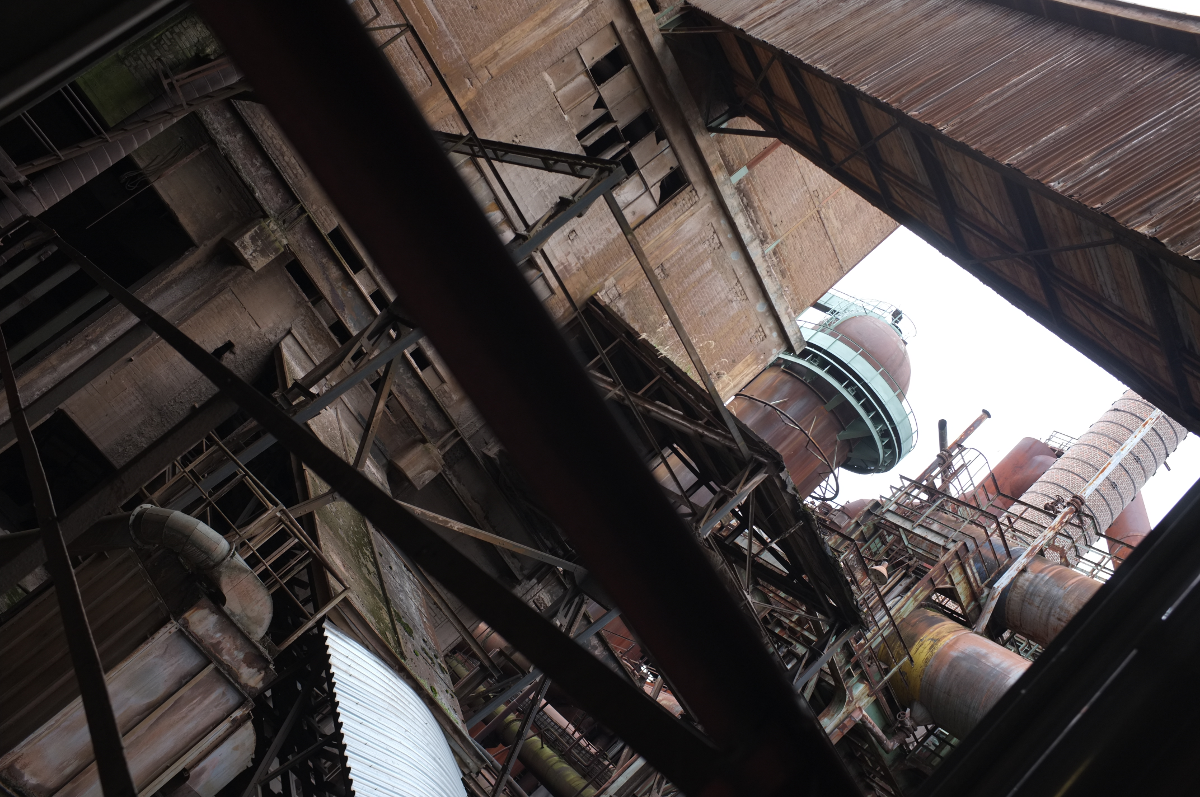
\includegraphics[width=0.7\textwidth]{Examples/example_5.png}
  \caption{Erstes Bild, V�lklinger H�tte}
  \label{fig:Huette}
\end{figure}

\subsection{Es geht besser}

Abbildung \ref{fig:Huette} ist zwar ganz nett anzusehen, aber vielleicht s�he es eleganter aus, wenn die Abbildung 
von unserem Textabschnitt umflossen wird.


\blindtext
\begin{wrapfigure}{l}{0.5\textwidth}
  \centering
  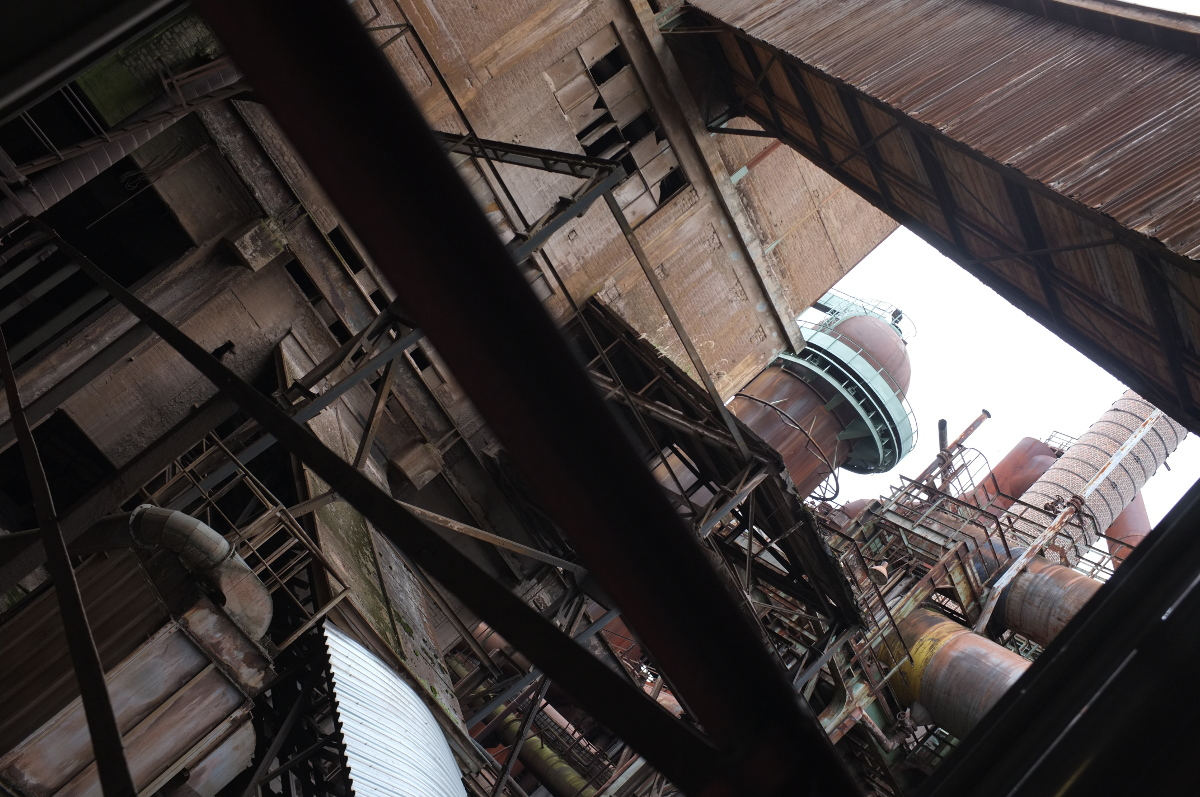
\includegraphics[width=0.5\textwidth]{Examples/example_5.jpg}
  \caption{V�lklinger H�tte, *.jpg}
  \label{fig:Huette2}
\end{wrapfigure}
\blindtext
\blindtext

\subsection{Mehrere Abbildungen nebeneinander}

Es ist ebenso m�glich mehrere Abbildungen nebeneinander zu setzen, wie in Abbildung \ref{fig:Beide} zu sehen ist.

\begin{figure}
  \subfloat[Erstes ...]{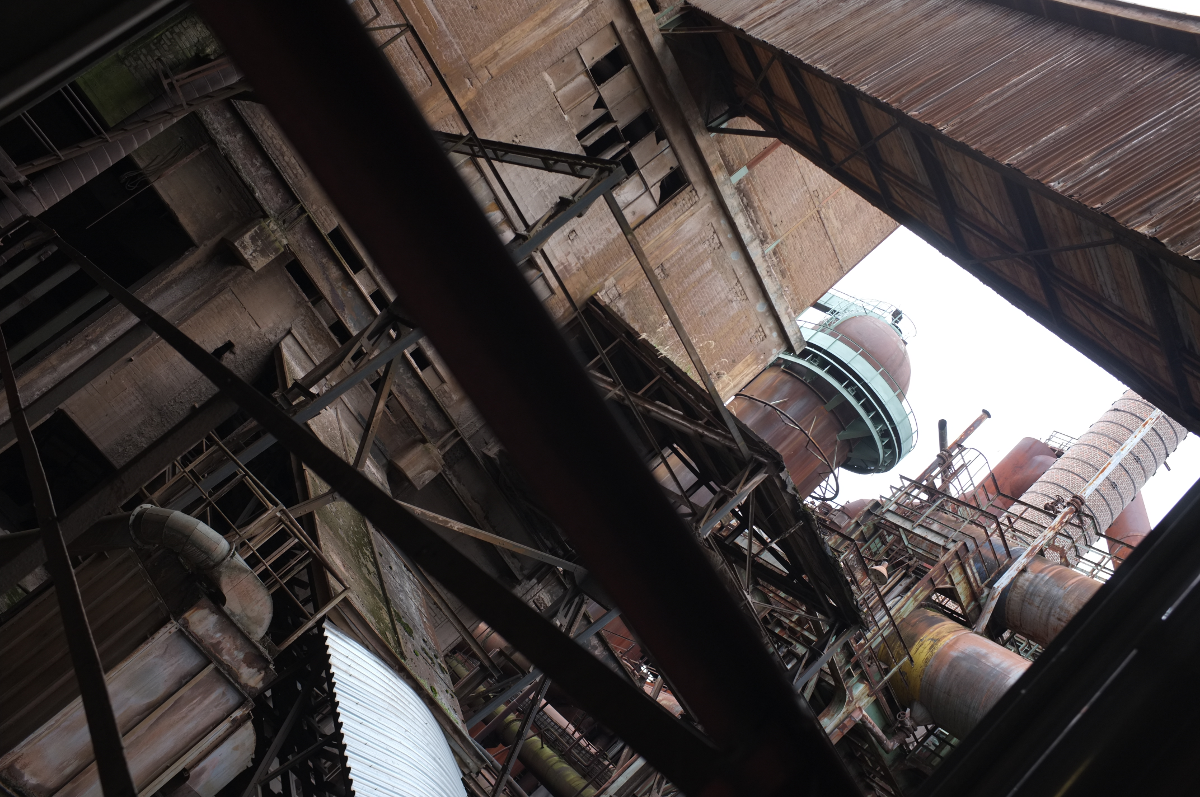
\includegraphics[width=0.49\textwidth]{Examples/example_5.png}}\hfill
  \subfloat[... und zweites Bild]{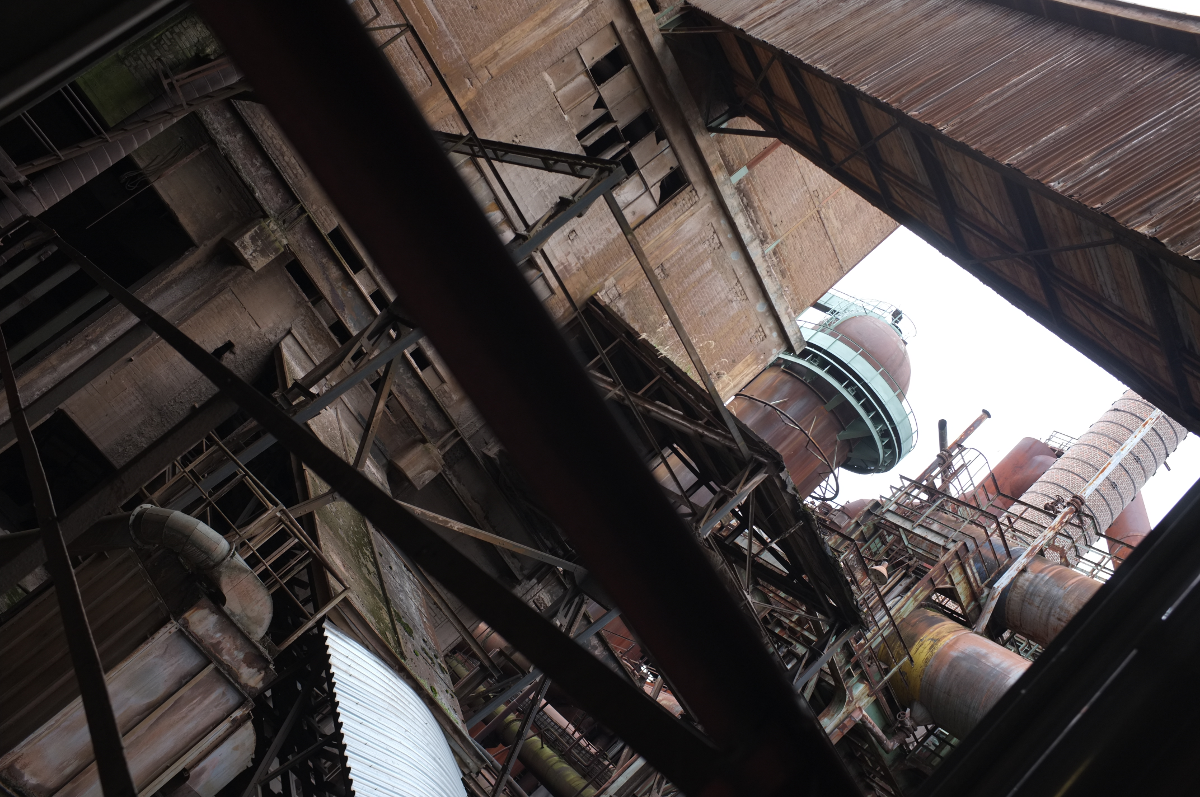
\includegraphics[width=0.49\textwidth]{Examples/example_5.png}}
  \caption{Abbildung \ref{fig:Huette} und \ref{fig:Huette2} nebeneinander}
  \label{fig:Beide}
\end{figure}


%*******************************
% 			Listings 		   *
%*******************************

\chapter{Quellcode einbinden}
Das Package \textit{lstlisting} ermöglicht es, Quellcode ansprechend in das Dokument einzubinden. Man kann Quellcode einzeilig einbinden, mittels \lstinline{\lstinline|Quellcode|}. Dabei ist darauf zu achten, dass der Befehl einmal mit \{ \} und einmal mit | | aufgerufen werden kann, je nachdem, welche Zeichen im angegebenen Quelltext genutzt werden. 
Es ist auch möglich eine eigene Umgebung für Quelltext zu schaffen:\\

\begin{lstlisting}[caption=Erstes Listing]
private Umgebung(int i, int k)
{
	System.out.println("Eine Funktion mit " + i + "und" + k ".");
}
\end{lstlisting}  

Wer Quelltext aus externen Dateien einbinden möchte, geht wie folgt vor:\\

\lstinputlisting
[caption={Externer Quellcode}]
{Examples/Code.java}

Wie genau der Quellcode formatiert und gefärbt ist, ist in \textit{htwsaar.i.mst.config.tex} hinterlegt.
\section{Mathematische Ausdr�cke}
\subsection{Allgemeines}
%********************************************

Mathematische Ausdr�cke sind eine kleine Kunst f�r sich. Am allereinfachsten kann man eine Formel, wie \(a + b = c\) in den Flie�text einbinden, wobei Latex die H�he der Ausdr�cke der Zeile an passt, wie hier zu sehen \(\sum_{y=0}^{x} a\) . In einer Umgebung sieht das schon anders aus:

\begin{equation}
  \sum_{y=0}^{x} a
\end{equation}

\subsection{Mathematisches}
\subsection{Br�che}
%********************************************

\begin{equation}
Ergebnis = \frac{a}{b}
\end{equation}

\begin{equation}
\frac{\sin{\alpha}^2 + \cos{\alpha}^2}{1} = 1
\end{equation}

\begin{equation}
\frac{-9x}{\frac{2y}{3z+2}}
\end{equation}

\subsection{Hoch- bzw. Tiefstellungen}
%********************************************

\begin{equation}
x_{i,j}^2
\end{equation}

\begin{equation}
{x_{i,j}}^2
\end{equation}

\begin{equation}
x_{n_0}
\end{equation}

\subsection{Text innerhalb von Formeln}
%********************************************

\begin{equation}
\sum_{y=1}^{n} y = \frac{n*(n+1)}{2}
\quad
\text{Gaus'sche Summenformel}
\end{equation}

\subsection{Matrizen}
%********************************************

Matrizen werden innerhalb der mathematischen Umgebung als wiederum neue Umgebung eingebunden. Wie bei Tabellen auch werden Zeilen durch \lstinline{\\} und Spalten durch \lstinline{&} getrennt.

\begin{equation}
\begin{pmatrix} 
a&b\\
c&d 
\end{pmatrix}
\end{equation} 

\begin{equation}
\begin{vmatrix} 
a&b\\
c&d 
\end{vmatrix}
\end{equation} 

\subsection{Fallunterscheidung}
%********************************************

\begin{equation}
f(x) = 
\begin{cases}
0, &\text{falls } x < 0 \\
1, &\text{falls } x \geq 0
\end{cases}
\end{equation}

\subsection{Ein paar griechische Buchstaben}
%********************************************

\begin{equation}
\alpha\beta\gamma\delta\epsilon\varepsilon\zeta\eta
\theta\iota\kappa\lambda\mu\nu\xi\pi\varpi\rho\varrho
\sigma\tau\upsilon\phi\varphi\chi\psi\omega
\end{equation}


% Eigene Shortcuts fuer laengere Befehle
\newcommand{\todox}[1]{\todo[inline, size=\small]{#1}}

%Nummerierte Anmerkungen
\newcounter{todocounter}

\renewcommand{\todox}[2][]{\stepcounter{todocounter}\todo[inline, size=\small,caption={\thetodocounter: #2}, #1]{\renewcommand{\baselinestretch}{0.5}\selectfont\thetodocounter: #2\par}}

%############################################################

\chapter{To-Do-Notes}


Lorem ipsum dolor sit amet, consectetuer adipiscing elit. Nulla
\todo{Plain todonotes.}%
urna. Maecenas interdum nunc in augue. Mauris quis massa in ante
tincidunt mollis. Proin imperdiet. Donec porttitor pede id est. Sed
in ante. Integer id arcu. Nam lectus nisl, posuere sit amet,
imperdiet ut, tristique ac, lorem. In erat. In commodo enim.
\todo[color=blue!40]{Todonote with a different color.}%
Phasellus libero ipsum, tempor a, pharetra consequat, pellentesque
sit amet, sem. Praesent ut augue luctus elit adipiscing ultricies.
Vestibulum suscipit cursus leo. Nullam molestie justo.


Morbi dui. Morbi convallis mi sed sem. Nulla convallis lacus vitae
risus. Phasellus adipiscing. Nullam tortor. Sed laoreet aliquam
ante. Vestibulum diam. Pellentesque nec leo. Pellentesque velit.
\todo[nolist]{Todonote that is only shown in the margin and not in
the list of todos.}%
Praesent congue mi eu ipsum cursus fringilla. Etiam leo erat,
tristique et, pharetra eget, mollis vitae, velit. In hac habitasse
\todo[size=\small, color=green!40]{A note with a small fontsize.}%
platea dictumst. In quam nibh, facilisis et, laoreet non, facilisis
tempus, justo.

\todo[inline]{A very long todonote that certainly will fill more
than a single line in the list of todos. Just to make sure let's add
some more text \ldots}

Donec nulla lectus, faucibus sit amet, auctor non, consectetuer
quis, pede. Nullam dictum. Nullam suscipit, ligula in scelerisque
\todo[noline]{A note with no line back to the text.}%
posuere, sapien purus rutrum magna, vitae pharetra leo quam vel
tortor. Donec eleifend condimentum sapien. Etiam sed orci. Aliquam
\todo[inline, color=red!50]{Inline todonotes.}%
tempor. Pellentesque egestas tortor id eros. Donec mauris justo,
commodo id, pellentesque id, eleifend non, mi. Duis venenatis
\todo[caption={A short entry in the list of todos}]{A very long
todonote that certainly will fill more than a single line in the
list of todos \ldots}
sagittis metus. 

\clearpage

\missingfigure{A figure I have to make \ldots}

%Nummerierte ToDo-Notes
\todox{Erste Nummer...}

\missingfigure[figwidth=\textwidth]{A figure I have to make \ldots}

\todox{Zweite Nummer...}

\clearpage

%Alles To-Do's als Liste ausgegeben
\listoftodos


 		% Abschlussarbeit geht!
%\include{Chapters/KapitelBachelorarbeit} <<< Hier alle Chapter der Abschlussarbeit (einzeln) einbinden

%********************************************************************
% Other Stuff in the Back
%*******************************************************
\cleardoublepage%********************************************************************
% Bibliography
%*******************************************************
\printbibliography

% ********************************************************************
% Appendix/Anhang
%***************************************************************
\appendix
\part*{Anhang}
\cleardoublepage%********************************************************************
% Appendix
%*******************************************************
\chapter{Erster Abschnitt}
In den Anhang geh�ren "`Hintergrundinformationen"', also weiterf�hrende Information, ausf�hrliche Listings, Graphen, Diagramme oder Tabellen, die den Haupttext mit detaillierten Informationen erg�nzen. 

\blindtext
\blindtext
\blindtext



%*******************************************************
\cleardoublepage\pagestyle{empty}

\hfill

\vfill

\pdfbookmark[0]{Kolophon}{colophon}
\section*{Kolophon}
Dieses Dokument wurde mit der \LaTeX-Vorlage f�r Abschlussarbeiten an der htw saar im Bereich Informatik/Mechatronik-Sensortechnik erstellt (\currentVersion). Die Vorlage wurde von Yves Hary und Andr\'e Miede entwickelt (mit freundlicher Unterst�tzung von Thomas Kretschmer und Helmut G. Folz).

\end{document}
% ********************************************************************
